\chapter{Introduction to Computer Design}

\section{Sistemi Embedded e Classi di Parallelismo}

Nel panorama odierno, il mercato dei calcolatori non è uniforme. Troviamo diverse tipologie di sistemi, tra cui i \textbf{sistemi embedded}, i quali sono onnipresenti (dal settore \textit{automotive} agli elettrodomestici, fino alle missioni aerospaziali).
I problemi nel mondo \textit{embedded} vengono spesso risolti ricorrendo a una delle seguenti soluzioni:
\begin{itemize}
    \item \textbf{Processore standard + logica custom + software custom}
    \item \textbf{Processore standard + software custom}
    \item \textbf{DSP (Digital Signal Processor) standard + software custom}
\end{itemize}
In questo contesto, i dispositivi programmabili come le \textbf{FPGA} (Field Programmable Gate Arrays) stanno giocando un ruolo sempre più rilevante, anche grazie alla loro capacità di essere riprogrammate sul campo per correggere eventuali guasti (come avviene nei satelliti).

\subsection{Classi di Parallelismo}
Per soddisfare l'enorme richiesta di prestazioni, le architetture sfruttano diverse tipologie di parallelismo:
\begin{itemize}
    \item \textbf{Data-level Parallelism (DLP):} Molti dati vengono elaborati contemporaneamente (es. applicare lo stesso filtro a tutti i pixel di un'immagine).
    \item \textbf{Task-level Parallelism (TaskLP):} Diversi task o processi operano in maniera indipendente (es. le richieste indipendenti di vari utenti su un server).
\end{itemize}

Queste classi di parallelismo vengono sfruttate da diverse architetture hardware:
\begin{enumerate}
    \item \textbf{Instruction-level Parallelism (ILP):} Sfrutta in modo modesto il DLP, eseguendo più istruzioni di un singolo flusso in parallelo (è il focus principale per i processori general-purpose, ad esempio tramite la \textit{pipeline}).
    \item \textbf{Vector Architectures e GPU:} Sfruttano massicciamente il DLP.
    \item \textbf{Thread-level Parallelism (TLP):} Sfrutta sia il DLP che il TaskLP, tipico dei sistemi multicore.
    \item \textbf{Request-level Parallelism (RLP):} Sfrutta il parallelismo a livello di richiesta, tipico dei cluster o dei server.
\end{enumerate}

\section{Architettura dei Calcolatori e Requisiti}
Negli ultimi decenni, il design dei calcolatori ha tratto grande vantaggio dalle innovazioni architetturali. Il divario di prestazioni tra i processori odierni e quelli passati sarebbe impossibile da giustificare unicamente con il miglioramento tecnologico dei semiconduttori (Legge di Moore).

L'architettura dei calcolatori comprende tre aspetti fondamentali:
\begin{enumerate}
    \item \textbf{Instruction Set Architecture (ISA):} L'interfaccia hardware/software (quali istruzioni la CPU può eseguire).
    \item \textbf{Organization:} L'organizzazione interna (come i moduli sono interconnessi, ad esempio le gerarchie di memoria o la logica di controllo).
    \item \textbf{Hardware:} L'implementazione fisica e la tecnologia manifatturiera.
\end{enumerate}

Il progettista (\textit{computer architect}) deve bilanciare cinque vincoli fondamentali: \textbf{Requisiti funzionali, Prezzo, Potenza (Power), Prestazioni (Performance) e Affidabilità (Dependability)}.

\subsection{La Legge di Moore}
\begin{definition}[Legge di Moore]
Il numero di dispositivi (ovvero di transistor) che possono essere integrati in un singolo chip raddoppia ogni 18-24 mesi.
\end{definition}
Nonostante le difficoltà fisiche nel scendere sotto la soglia dei nanometri, le aziende continuano a innovare, per esempio esplorando design tridimensionali, accatastando strati di silicio per mantenere alto il numero di transistor riducendo l'area bidimensionale.

\begin{figure}[H]
    \centering
    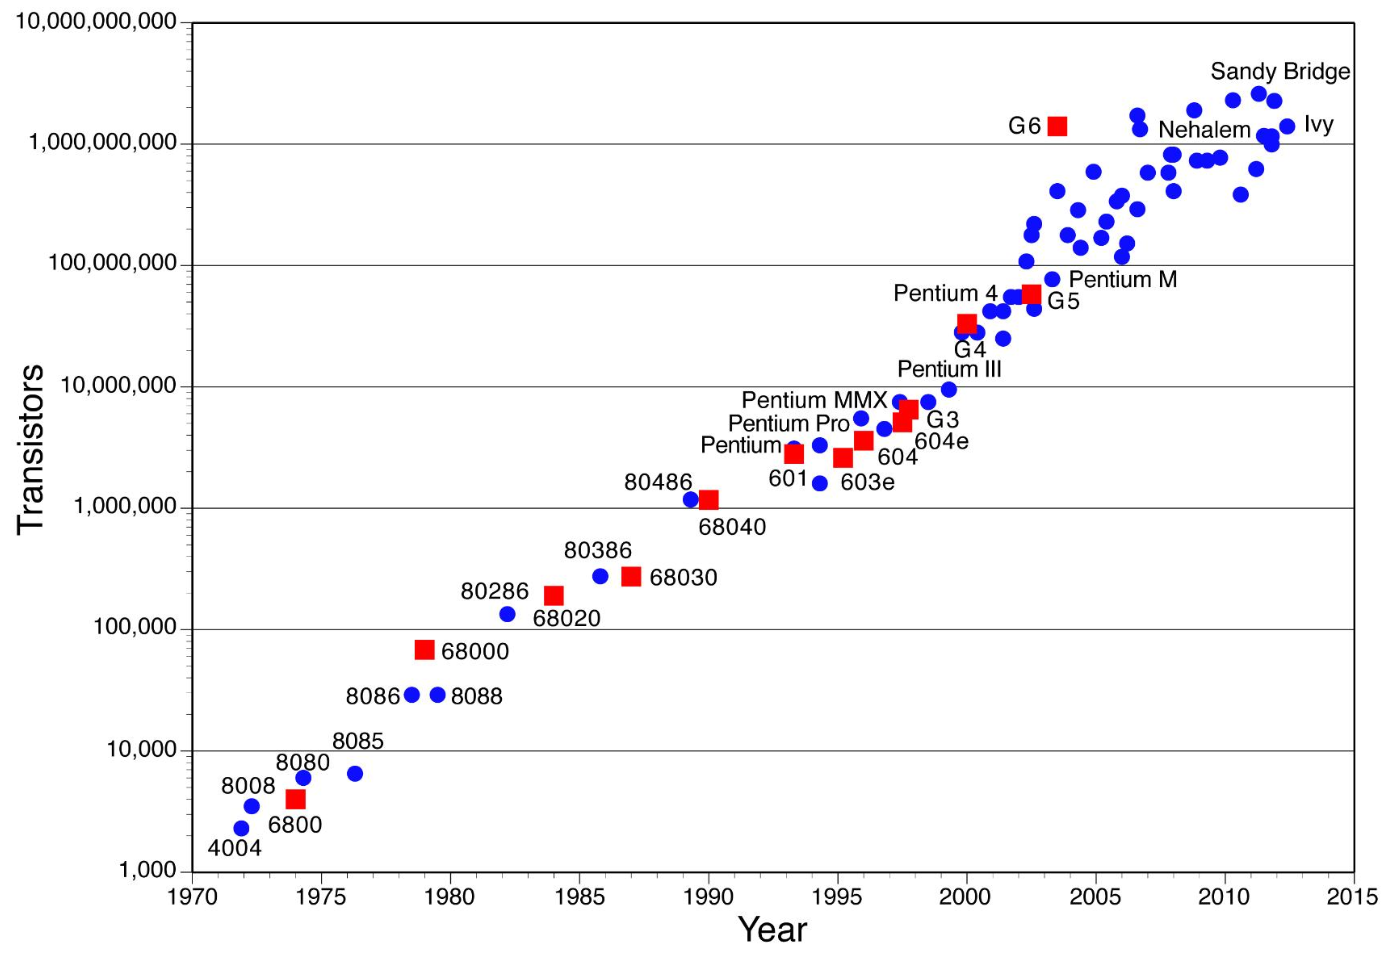
\includegraphics[width=0.9\textwidth]{capitoli/01_computer_design_introduction/images/image.png}
    \caption{Crescita della complessità dei processori Intel nel corso degli anni.}
    \label{fig:moore}
\end{figure}

\section{Affidabilità (Dependability) e Sicurezza}
L'affidabilità è diventata cruciale, specialmente in contesti \textit{safety-critical} come la guida autonoma, i sistemi spaziali o semplicemente per garantire che i server cloud non producano calcoli errati.
I guasti possono essere causati da bug hardware (es. il noto baco del divisore nel Pentium 4), difetti di produzione o semplice invecchiamento (usura) del silicio.

\subsection{Metriche di Affidabilità}
Per quantificare l'affidabilità si usano diverse metriche statistiche:
\begin{itemize}
    \item \textbf{MTTF (Mean Time To Failure):} Il tempo medio previsto prima che si verifichi un guasto.
    \item \textbf{FIT (Failures In Time):} È il reciproco del MTTF. Viene definito come un guasto ogni miliardo di ore: \( 1 \text{ FIT} = \frac{1}{10^9 \text{ ore}} \).
    \item \textbf{MTTR (Mean Time To Repair):} Il tempo medio necessario per riparare il sistema una volta avvenuto il guasto (es. riconfigurando una FPGA in un satellite da remoto).
    \item \textbf{MTBF (Mean Time Between Failures):} Il tempo medio tra due guasti successivi, calcolato come:
    \[ \text{MTBF} = \text{MTTF} + \text{MTTR} \]
\end{itemize}

L'\textbf{Availability} (Disponibilità) è definita come la probabilità che un sistema funzioni correttamente in un istante di tempo generico.

\begin{remark}[Perché 1 FIT non è trascurabile?]
Un valore di 1 FIT (un guasto ogni miliardo di ore) sembra eccellente se riferito a una singola persona. Tuttavia, su larga scala, il problema emerge chiaramente. Se in Europa circolano centinaia di milioni di auto, e ciascuna possiede decine di dispositivi elettronici, la somma totale delle ore operative è gigantesca. Statisticamente, questo significa avere un dispositivo che fallisce ogni 2-5 ore nell'intero parco auto europeo. Per questo motivo, industrie come STMicroelectronics puntano allo \textbf{Zero FIT}.
\end{remark}

\subsection{La Curva a Vasca (Bathtub Curve) e il Burn-in}
Il ciclo di vita dei guasti hardware segue tipicamente una "Bathtub curve" (curva a vasca da bagno):

    \begin{figure}[H]
        \centering
        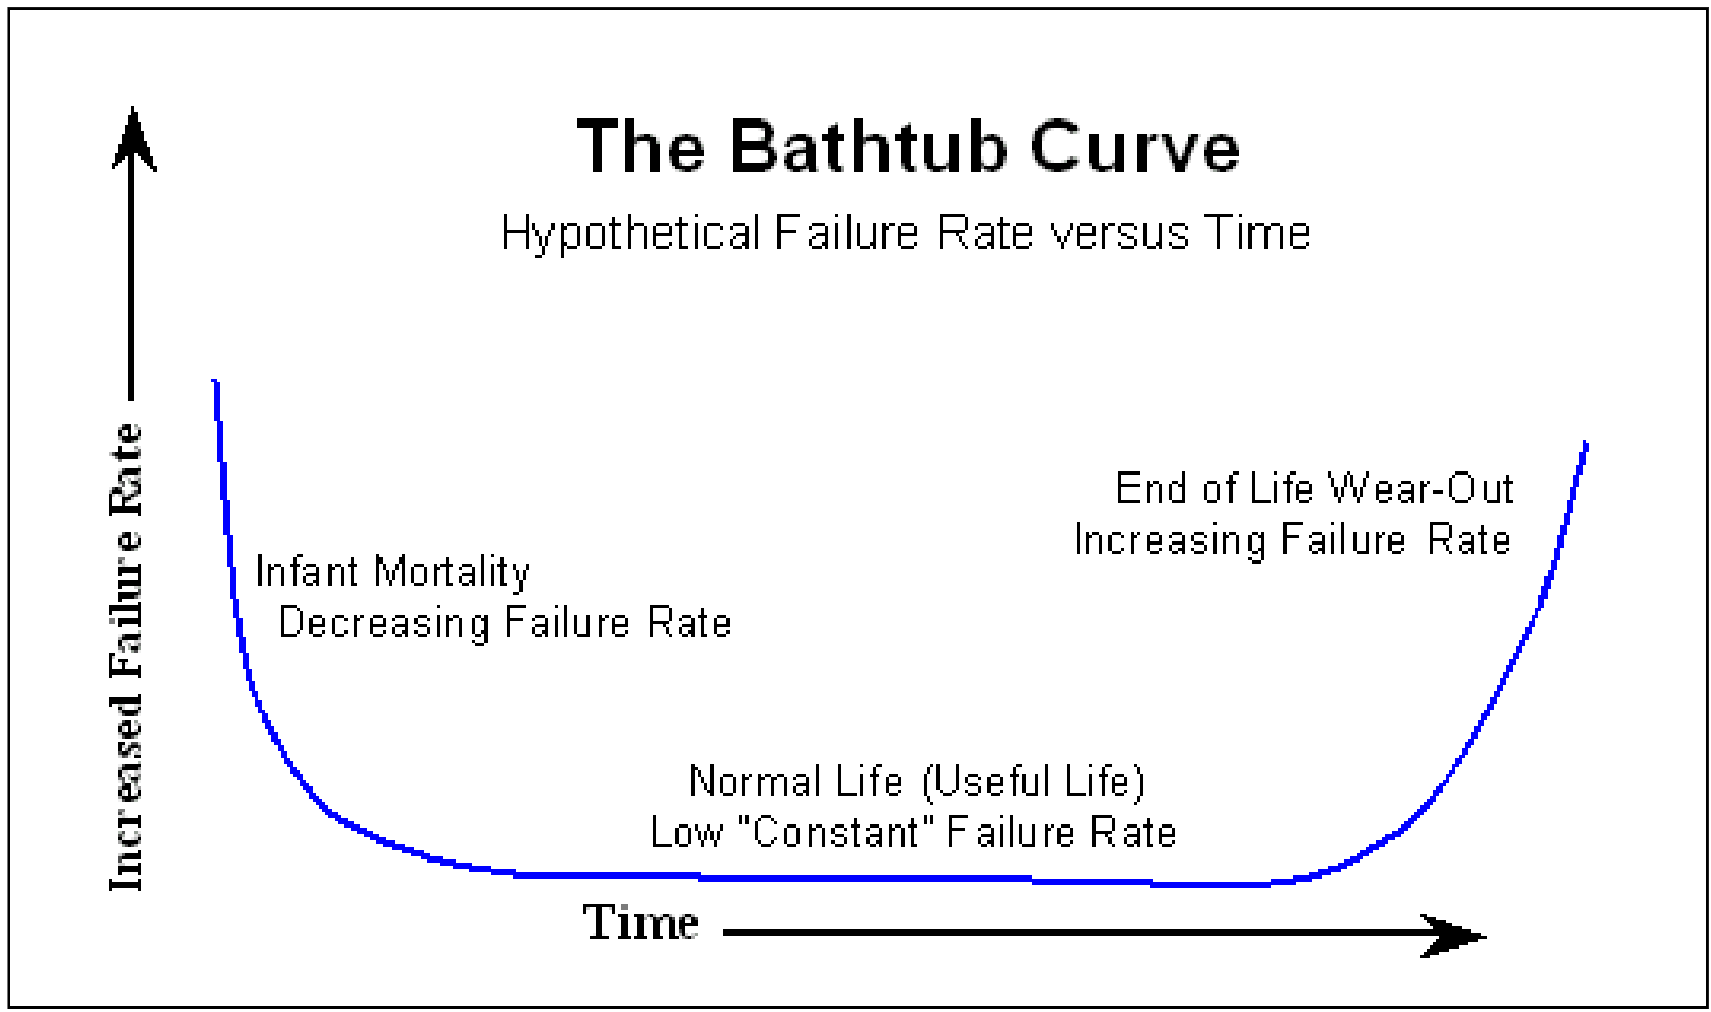
\includegraphics[width=0.6\textwidth]{capitoli/01_computer_design_introduction/images/bathtube.png}
        \caption{Curva a vasca (Bathtub Curve) del ciclo di vita dei guasti hardware.}
        \label{fig:bathtub}
    \end{figure}

\begin{enumerate}
    \item \textbf{Mortalità infantile:} Subito dopo la fabbricazione, il tasso di guasti è altissimo a causa dei difetti di produzione non rilevati (yield basso).
    \item \textbf{Vita utile:} Il tasso si abbassa e rimane stabile per molti anni (10-15 anni).
    \item \textbf{Invecchiamento (Wear-out):} Alla fine del ciclo vitale, l'usura fisica del silicio fa rialzare bruscamente la curva dei guasti.
\end{enumerate}

Per evitare di vendere dispositivi soggetti a "mortalità infantile", i produttori utilizzano la tecnica del \textbf{Burn-in test}. I chip appena prodotti vengono inseriti in forni industriali ad alte temperature ed eseguiti sotto forte stress di calcolo per alcune ore. Questo processo simula anni di vita operativa; i chip che sopravvivono al \textit{burn-in} sono considerati stabili ed entrano direttamente nella fase di "vita utile".

\section{Valutazione delle Prestazioni (Performance Evaluation)}
Le prestazioni possono essere definite in modi diversi in base a chi osserva:
\begin{itemize}
    \item L'\textbf{utente} valuta il \textbf{Response Time} (o tempo di esecuzione): il tempo trascorso dalla richiesta di esecuzione fino alla sua conclusione.
    \item Il \textbf{manager/amministratore} valuta il \textbf{Throughput}: la quantità totale di lavoro (es. istruzioni al secondo) completata in una data unità di tempo.
\end{itemize}

\subsection{I Benchmark}
Il tempo di esecuzione andrebbe misurato idealmente con il \textit{workload} (carico di lavoro) reale dell'utente. Poiché questo varia da utente a utente, l'industria adotta i \textbf{Benchmark}, insiemi di programmi appositamente selezionati per simulare casi d'uso reali. Esistono diverse categorie:
\begin{itemize}
    \item \textbf{Real programs:} Programmi veri e propri (compilatori C, processori di testo).
    \item \textbf{Kernels:} Piccoli frammenti di codice molto intensivi (es. Linpack).
    \item \textbf{Toy benchmarks:} Algoritmi classici come Quicksort o il Crivello di Eratostene.
    \item \textbf{Synthetic benchmarks:} Codice creato artificialmente per stressare componenti specifiche (es. Whetstone).
\end{itemize}

Tra i più noti ricordiamo le suite dello \textbf{SPEC} (Standard Performance Evaluation Corporation) per processori general purpose, e \textbf{MiBench} per il mondo dei dispositivi embedded, che raccoglie programmi specifici per ambiti come Automotive, Network e Sicurezza.

\begin{remark}[La Riproducibilità]
Qualsiasi misurazione tramite benchmark deve garantire la \textbf{riproducibilità}. Chi testa deve dichiarare esplicitamente: le caratteristiche dell'hardware (configurazione del sistema), il software (Sistema Operativo e Compilatore usato) e i precisi dati in input passati al programma (es. dimensione della matrice per il Quicksort), altrimenti i risultati sono inaffidabili.
\end{remark}

\subsection{Metriche di Confronto: Media Aritmetica e Pesata}
Per confrontare le prestazioni di un processore \( X \) rispetto a un processore \( Y \) (spesso normalizzati rispetto a una macchina di riferimento), usiamo diverse tipologie di medie applicate sui tempi di esecuzione di un insieme di \( n \) benchmark.

La \textbf{Media Aritmetica} assume che tutti i benchmark siano eseguiti con la stessa frequenza:
\[ \text{Arithmetic Mean} = \frac{1}{n} \sum_{i=1}^{n} \text{Time}_i \]

Tuttavia, nella realtà, alcune applicazioni sono molto più usate di altre. È quindi più corretto utilizzare la \textbf{Media Aritmetica Pesata} (Weighted arithmetic mean), assegnando un peso (\( \text{Weight}_i \)) a ciascun programma, dove la somma dei pesi è uguale a 1.
\[ \text{Weighted execution time} = \sum_{i=1}^{n} \left( \text{Weight}_i \times \text{Time}_i \right) \]

\begin{example}[Impatto dei Pesi sulle Prestazioni]
Consideriamo due programmi (\(P1\) e \(P2\)), tre macchine (\(A, B, C\)) e tre set di pesi (\(W_1, W_2, W_3\)).
\begin{itemize}
    \item \( P1 \): La macchina A impiega 1s, B impiega 10s, C impiega 20s.
    \item \( P2 \): La macchina A impiega 1000s, B impiega 100s, C impiega 20s.
\end{itemize}
Consideriamo i tempi di esecuzione dei due programmi sulle tre macchine:
\begin{center}
\begin{tabular}{c|cc}
    & \(P1\) & \(P2\) \\
    \hline
    A & 1 s & 1000 s \\
    B & 10 s & 100 s \\
    C & 20 s & 20 s
\end{tabular}
\end{center}

\paragraph{Caso \(W_1\): pesi 0.50 e 0.50.}
In questo caso i due programmi hanno la stessa importanza. Il tempo medio pesato di ciascuna macchina è:
\begin{align*}
    T_A &= 0.50 \cdot 1 + 0.50 \cdot 1000 = 500.5\,\text{s}, \\
    T_B &= 0.50 \cdot 10 + 0.50 \cdot 100 = 55\,\text{s}, \\
    T_C &= 0.50 \cdot 20 + 0.50 \cdot 20 = 20\,\text{s}.
\end{align*}
Quindi la macchina \textbf{C} è la migliore, perché ha il tempo medio pesato più basso. Inoltre, è molto bilanciata: impiega 20 s per entrambi i programmi.

\paragraph{Caso \(W_3\): pesi 0.999 e 0.001.}
Ora quasi tutta l'importanza è assegnata a \(P1\), mentre \(P2\) conta soltanto per lo 0.1\%. I nuovi tempi medi pesati sono:
\begin{align*}
    T_A &= 0.999 \cdot 1 + 0.001 \cdot 1000 = 1.999\,\text{s} \approx 2\,\text{s}, \\
    T_B &= 0.999 \cdot 10 + 0.001 \cdot 100 = 10.09\,\text{s}, \\
    T_C &= 0.999 \cdot 20 + 0.001 \cdot 20 = 20\,\text{s}.
\end{align*}
In questo caso la macchina \textbf{A} è la migliore, perché è molto veloce su \(P1\), il programma che pesa quasi interamente sul risultato.

Il risultato cambia perché la macchina migliore dipende dal carico di lavoro considerato, cioè dalla frequenza con cui vengono eseguiti i programmi. Con \(W_1\), i due programmi contano allo stesso modo e vince la macchina C, più bilanciata. Con \(W_3\), conta quasi solo \(P1\) e vince la macchina A. Non esiste quindi una macchina ``migliore in assoluto'': la scelta dipende dai pesi assegnati ai programmi.
\end{example}

\section{Miglioramenti Architetturali}

Quando si ha l'opportunità di riprogettare una componente hardware per aumentare le prestazioni, è necessario poter valutare analiticamente la bontà della scelta. Due strumenti sono essenziali: la Legge di Amdahl e l'Equazione delle Prestazioni della CPU.

\subsection{La Legge di Amdahl}
La \textbf{Legge di Amdahl} calcola lo \textit{Speedup} (incremento di velocità) globale ottenibile migliorando solo una specifica frazione del sistema.
\[ \text{Speedup} = \frac{\text{Tempo originale}}{\text{Tempo migliorato}} \]

Definiamo due parametri:
\begin{itemize}
    \item \( F \) (Frazione migliorata): la porzione del tempo di esecuzione originale che beneficerà del miglioramento.
    \item \( S \) (Speedup della frazione): di quanto ho reso più veloce quella specifica frazione.
\end{itemize}

Il nuovo tempo di esecuzione sarà composto dal tempo per la porzione non migliorata \((1 - F)\) più il tempo per la porzione migliorata, ora diviso per lo speedup \(\frac{F}{S}\). 
La Legge di Amdahl è formulata come:
\begin{equation}
\text{Speedup Globale} = \frac{1}{(1 - F) + \frac{F}{S}}
\end{equation}

\begin{example}[Valutazione di due alternative con Amdahl]
Siamo di fronte a due possibili scelte di progettazione, ma per ragioni di budget possiamo implementarne solo una:
\begin{enumerate}
    \item \textbf{Miglioramento Radice Quadrata:} Velocizza le operazioni di radice quadrata di un fattore 10 (\( S = 10 \)). Queste operazioni rappresentano il 20\% del tempo del programma (\( F = 0.20 \)).
    \item \textbf{Miglioramento Floating Point globale:} Velocizza \textbf{tutte} le operazioni floating point di un fattore 2 (\( S = 2 \)). Queste operazioni rappresentano il 50\% del programma (\( F = 0.50 \)).
\end{enumerate}

Calcoliamo lo Speedup nei due casi:
\begin{align*}
\text{Speedup}_1 &= \frac{1}{(1 - 0.20) + \frac{0.20}{10}} = \frac{1}{0.80 + 0.02} = \frac{1}{0.82} \approx 1.22 \\
\text{Speedup}_2 &= \frac{1}{(1 - 0.50) + \frac{0.50}{2}} = \frac{1}{0.50 + 0.25} = \frac{1}{0.75} \approx 1.33
\end{align*}
Nonostante l'accelerazione nominale del primo modulo fosse enorme (10 volte più veloce), conviene implementare il secondo modulo (Speedup globale 1.33 contro 1.22), perché ha un impatto maggiore sull'esecuzione complessiva del programma.
\end{example}

\subsection{Equazione delle prestazioni della CPU}
In fase di simulazione e progettazione teorica, il tempo di CPU può essere approssimato dalla seguente equazione fondamentale:
\begin{equation}
\text{CPU Time} = \left( \sum_{i=1}^{n} \text{CPI}_i \times \text{IC}_i \right) \times \text{Clock cycle time}
\end{equation}
Dove:
\begin{itemize}
    \item \textbf{CPI\textsubscript{i} (Cycles Per Instruction):} Cicli di clock necessari per eseguire un'istruzione di tipo \( i \).
    \item \textbf{IC\textsubscript{i} (Instruction Count):} Numero di istruzioni di quel tipo effettivamente eseguite dal programma.
    \item \textbf{Clock cycle time:} Periodo del clock (inverso della frequenza, $T = \frac{1}{f}$).
\end{itemize}

\begin{remark}[Limitazioni dell'Equazione]
Nelle architetture moderne basate su \textit{pipeline}, calcolare analiticamente il CPI puro è molto difficile e impreciso. Il numero reale di cicli di clock richiesti da un'istruzione dipenderà dinamicamente da:
\begin{itemize}
    \item Dipendenze tra istruzioni contigue (es. stalli della pipeline).
    \item Comportamento della gerarchia di memoria (es. una \textit{cache miss} fermerà l'istruzione in attesa della memoria RAM centrale, variando enormemente i cicli richiesti).
\end{itemize}
Per ottenere dati affidabili è dunque necessario ricorrere a complessi simulatori software.
\end{remark}